\section*{Math 202A - Final Exam - Dan Davison - \texttt{ddavison@berkeley.edu}}

\begin{mdframed}
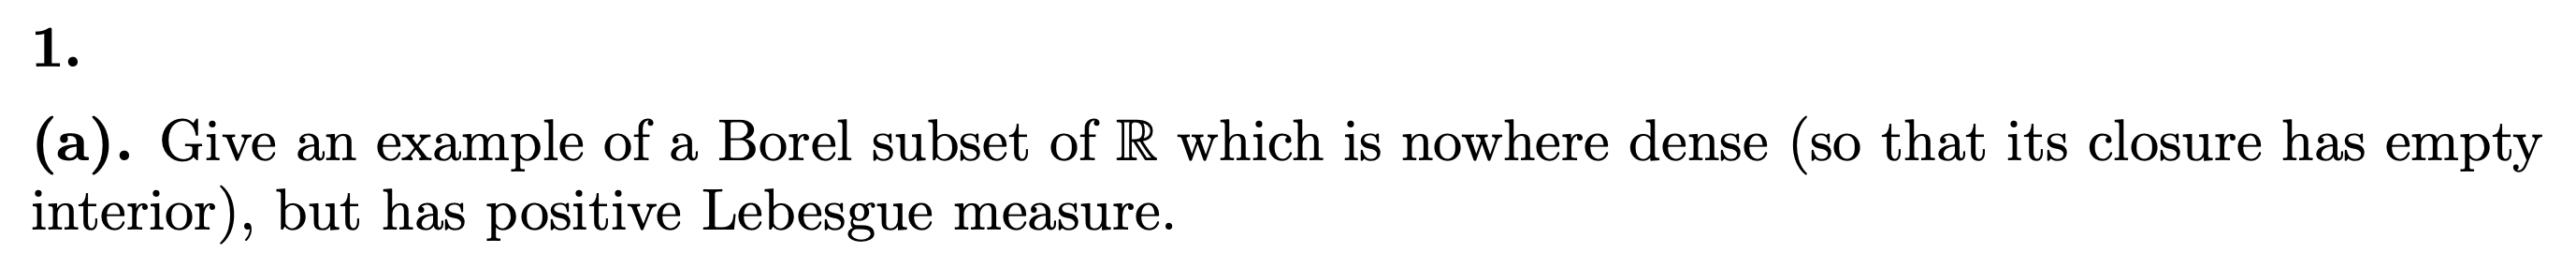
\includegraphics[width=400pt]{img/analysis--berkeley-202a-final-c9d2.png}
\end{mdframed}

\begin{proof}
  Fat Cantor set.
  \red{TODO}
\end{proof}

\begin{mdframed}
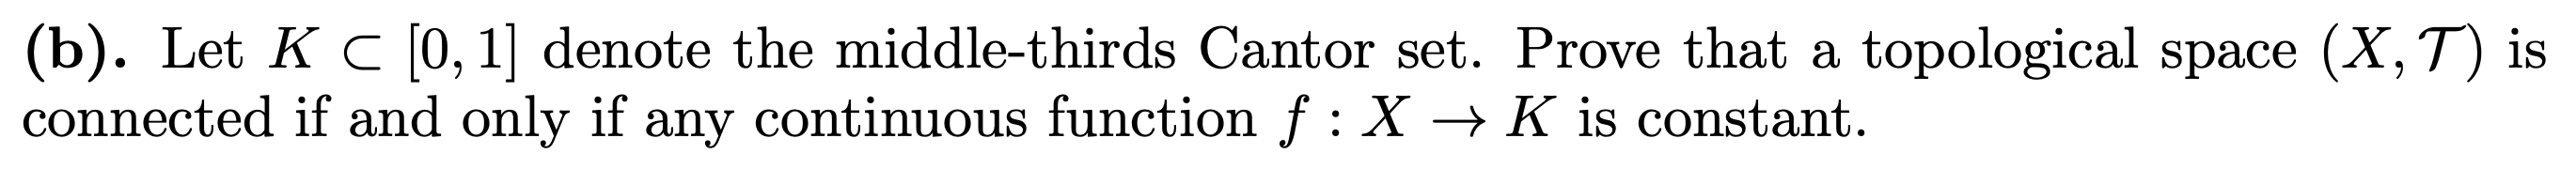
\includegraphics[width=400pt]{img/analysis--berkeley-202a-final-4333.png}
\end{mdframed}

\begin{proof}
  \red{TODO}
\end{proof}

\begin{mdframed}
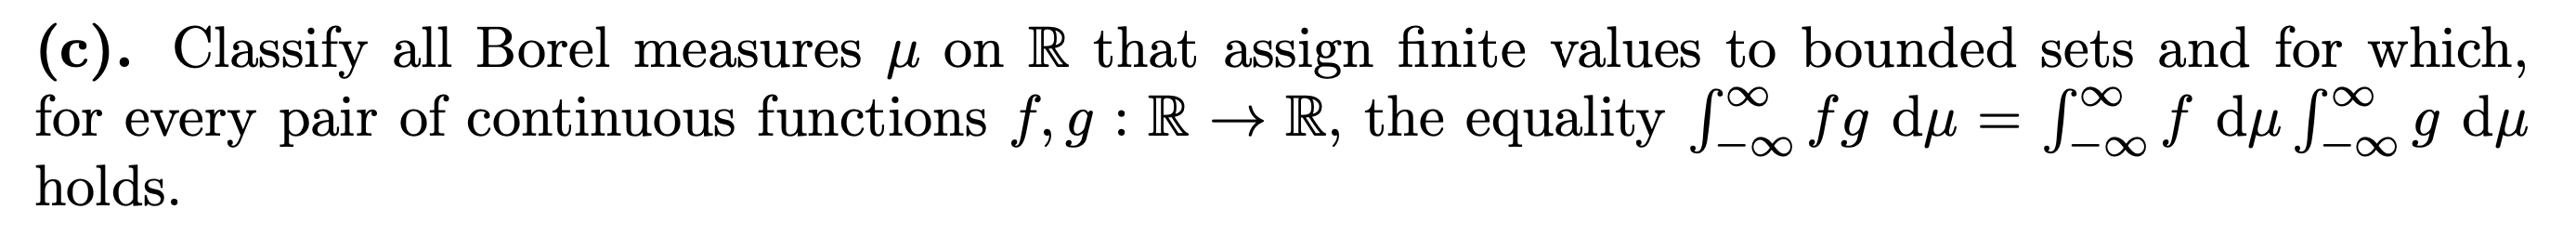
\includegraphics[width=400pt]{img/analysis--berkeley-202a-final-0bf8.png}
\end{mdframed}

\begin{proof}
  \red{TODO}
\end{proof}

\newpage
\begin{mdframed}
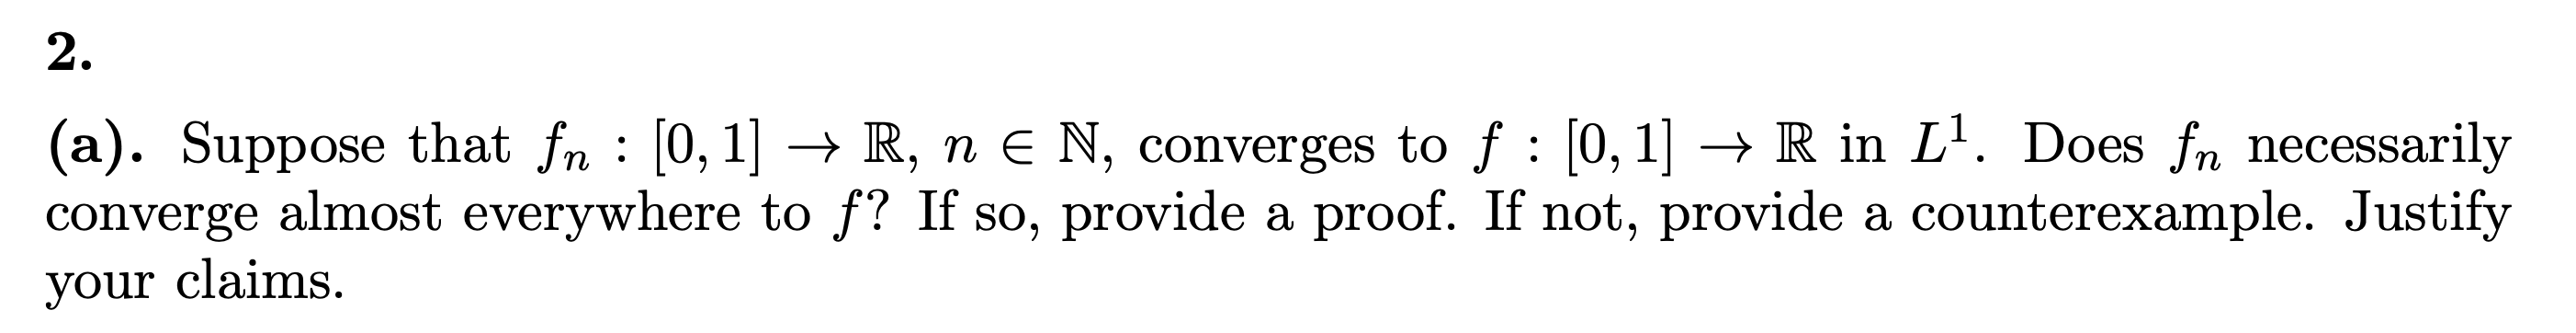
\includegraphics[width=400pt]{img/analysis--berkeley-202a-final-04b9.png}
\end{mdframed}

\begin{theorem}[Bass proposition 8.1]\label{bass-8.1}
  If $f$ is real-valued, non-negative, and measurable, and $\int f = 0$, then $f = 0$ a.e.
\end{theorem}

\begin{proof}
  Let $f_n: [0, 1] \to \R$, $n \in \N$, converge to $f: [0, 1] \to \R$ in $L^1$. Thus, by definition,
  \begin{align*}
    \limninf \int |f_n - f| = 0.
  \end{align*}
  We want to prove or disprove the statement
  \begin{align*}
    \limn f_n = f \ae
  \end{align*}
  Suppose we could bring the limit inside. Then
  \begin{align*}
    \int \limninf |f_n - f| = 0,
  \end{align*}
  therefore by Bass proposition 8.1 $\limninf |f_n - f| = 0$ a.e. and thus $f_n$ converges almost everywhere to $f$.

  But bringing the limit inside is justified by neither MCT nor DCT. So let's look for a counter-example based
  on not satisfying DCT conditions.

  \red{TODO}
\end{proof}

This is reminiscent of HW8 7.13

\begin{mdframed}
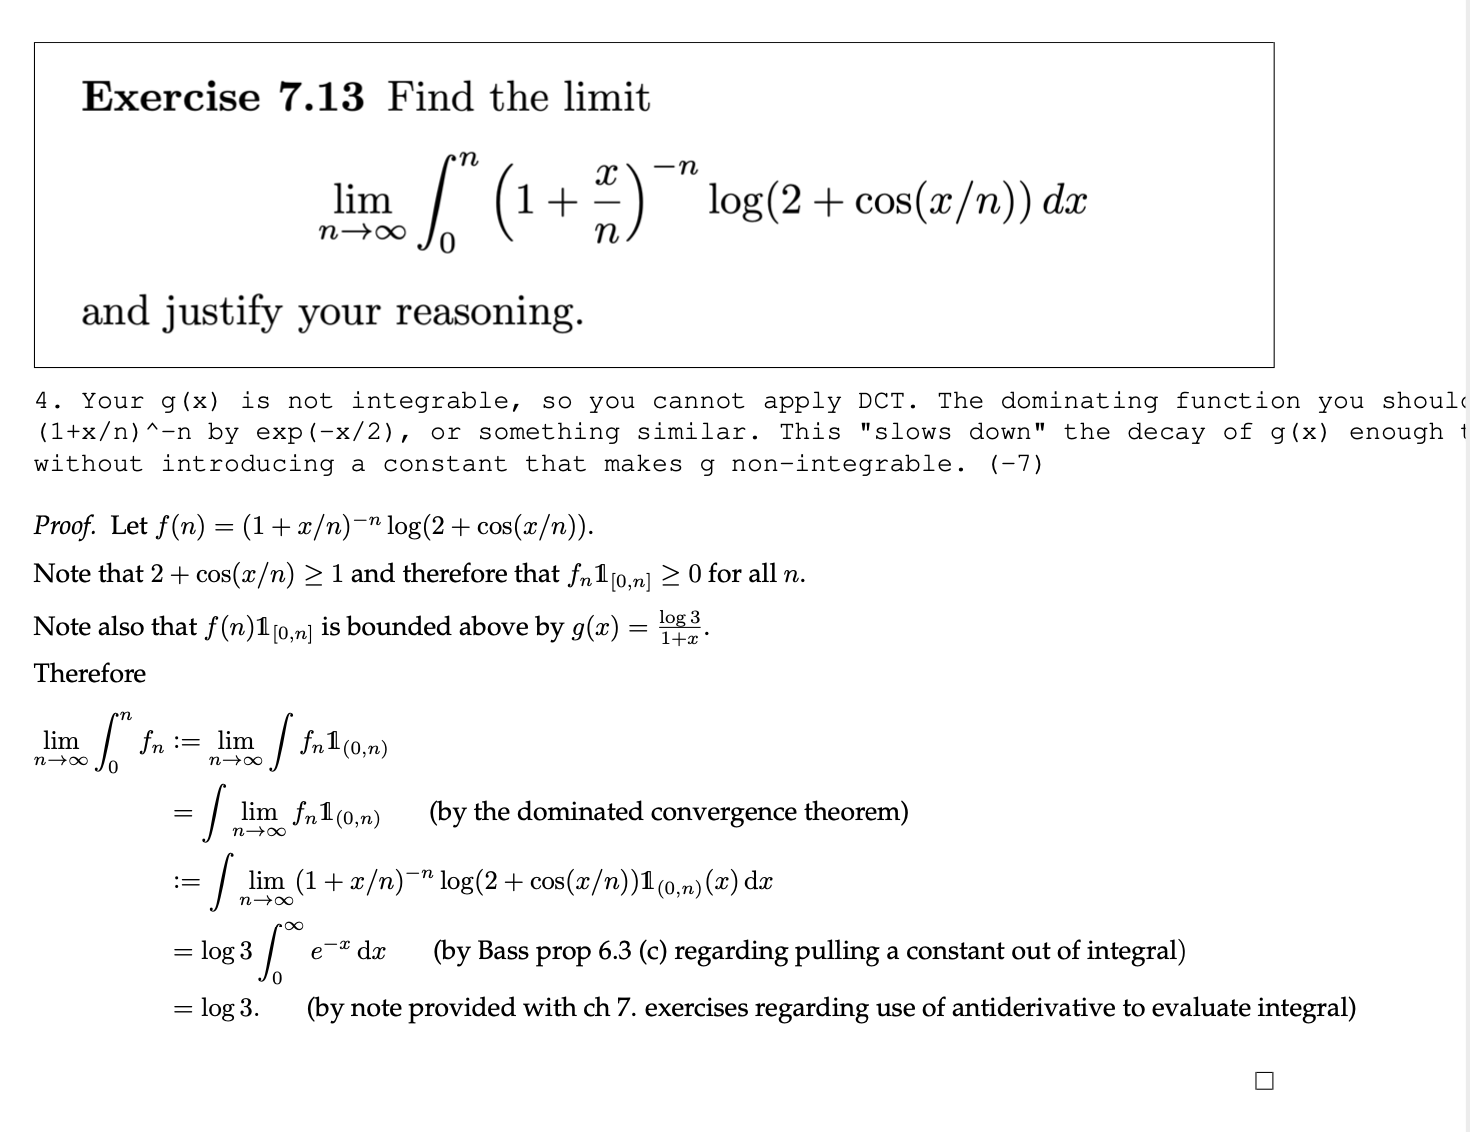
\includegraphics[width=400pt]{img/analysis--berkeley-202a-final-5921.png}
\end{mdframed}

\begin{mdframed}
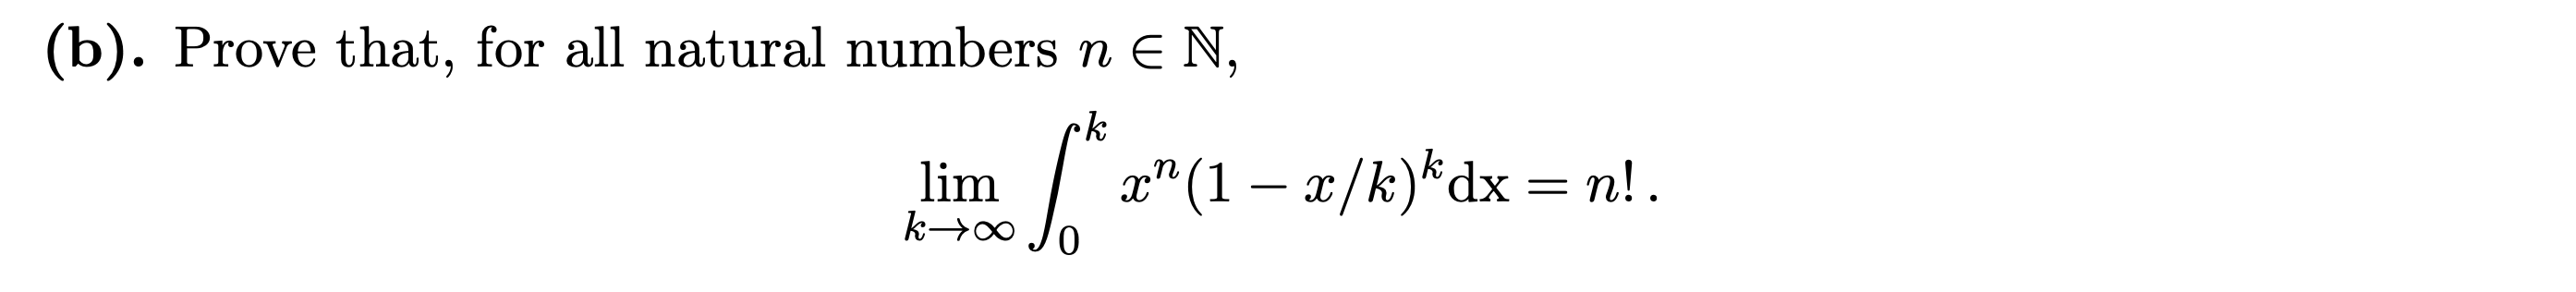
\includegraphics[width=400pt]{img/analysis--berkeley-202a-final-96cc.png}
\end{mdframed}

\begin{proof}
  Note that the integrand is non-negative.

  We want a dominating function. What about $x^ne^{-x/2}$? Is this integrable? It's continuous so we can use
  traditional Riemann / high-school integration techniques. I think it can be done by integration py parts and
  induction/recurrence.

  We may apply the DCT since the integrand is non-negative and bounded above by the integrable
  function $x^ne^{-x/2}$. Therefore
  \begin{align*}
    \lim_{k \to \infty} \int_0^k x^n (1 - x/k)^k \dx
    &= \int_0^k x^n \lim_{k \to \infty} (1 - x/k)^k \dx \\
    &= \int_0^k x^n e^{-x} \dx \\
  \end{align*}
  \red{TODO} how am I dealing with the $k$ in the upper integral bound?
\end{proof}

\begin{minted}{wolfram} :results latex
 Integrate[x^n * Exp[-x/2], {x, 0, Infinity}]
\end{minted}

\begin{align*}
\text{ConditionalExpression}\left[2^{n+1} \Gamma (n+1),\Re(n)>-1\right]
\end{align*}



\begin{mdframed}
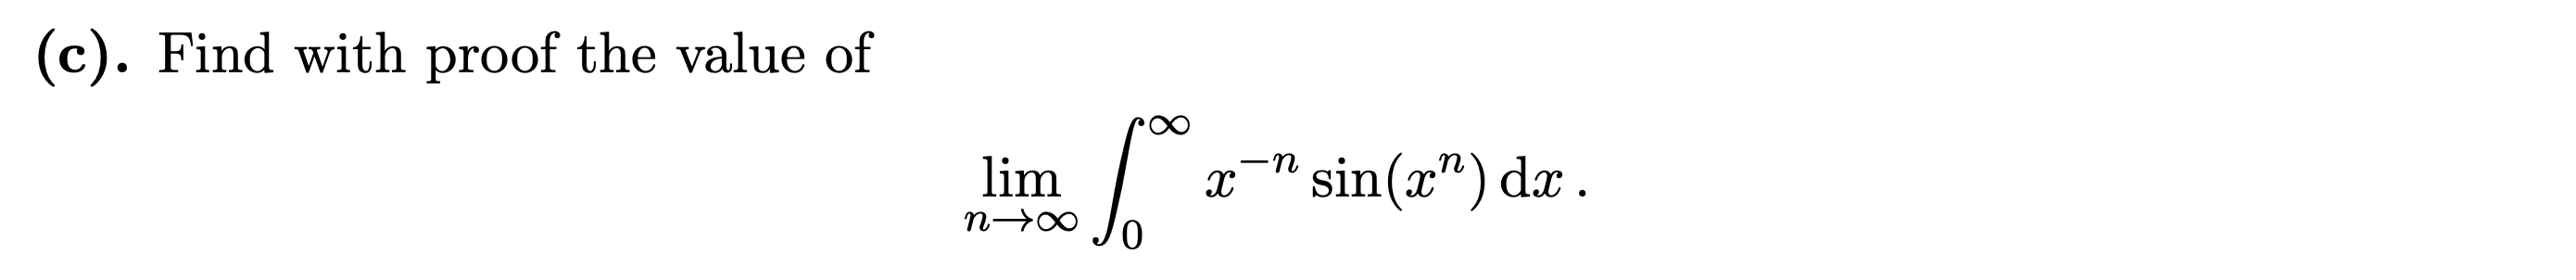
\includegraphics[width=400pt]{img/analysis--berkeley-202a-final-c137.png}
\end{mdframed}

\begin{proof}
  \red{TODO}
  bound the integral above?
\end{proof}


\newpage
\begin{mdframed}
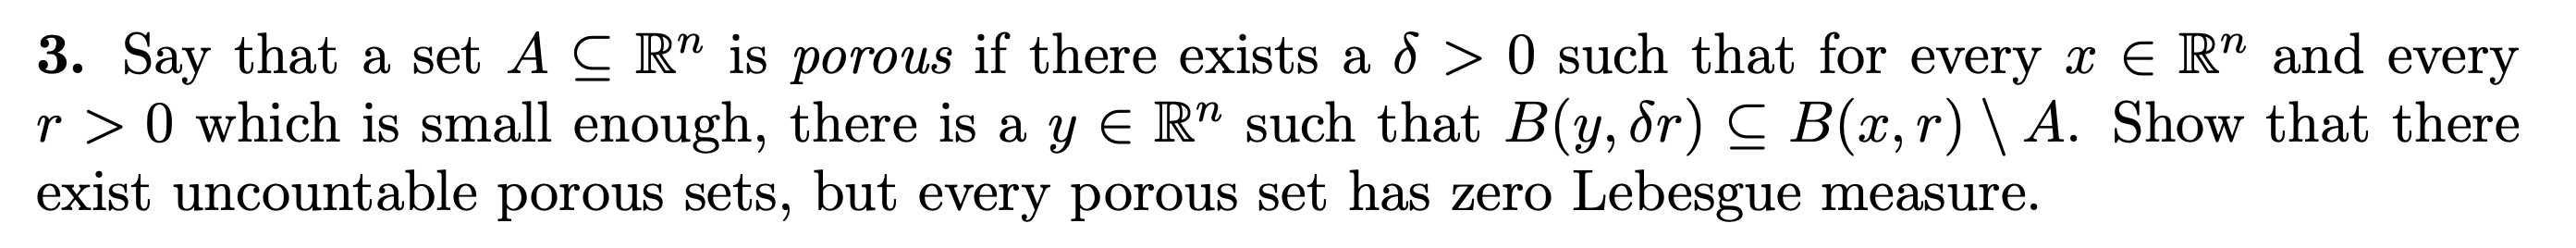
\includegraphics[width=400pt]{img/analysis--berkeley-202a-final-ef68.png}
\end{mdframed}

% I'm pretty sure how small r is should be independent of what x is, so you choose δ and r′ such that for every
% x and every r<r′, there exists y such that ...

% https://www.wikiwand.com/en/Porous_set
\begin{mdframed}
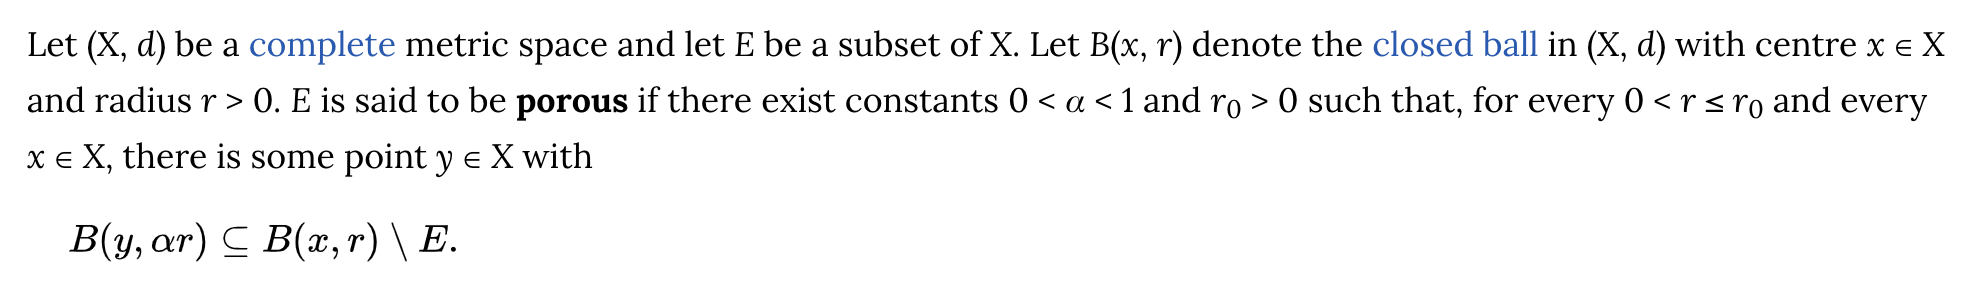
\includegraphics[width=400pt]{img/analysis--berkeley-202a-final-b463.png}
\end{mdframed}

\begin{proof}

  Notice that in the definition, the same $\delta$ and $r_0$ work everywhere:

  For every ball smaller than $r_0$, there exists a ball that is smaller still by a factor of $\delta$ that
  fits in the first ball and avoids every point of $A$.

  So consider an outer ball of size $r < r_0$. There exists an inner ball of size $\delta r$ that works.
  Furthermore this inner ball works for all larger outer balls.
\end{proof}

\begin{claim}
  The middle-thirds Cantor set is porous.

  This implies that there exist uncountable porous sets, since the middle-thirds Cantor set is uncountable.
\end{claim}

\begin{proof}

\end{proof}

\begin{claim}
  Every porous set has zero Lebesgue measure.
\end{claim}

\begin{proof}
  We must show that every porous set can be covered by a set of arbitrarily small measure.
\end{proof}



\newpage
\begin{mdframed}
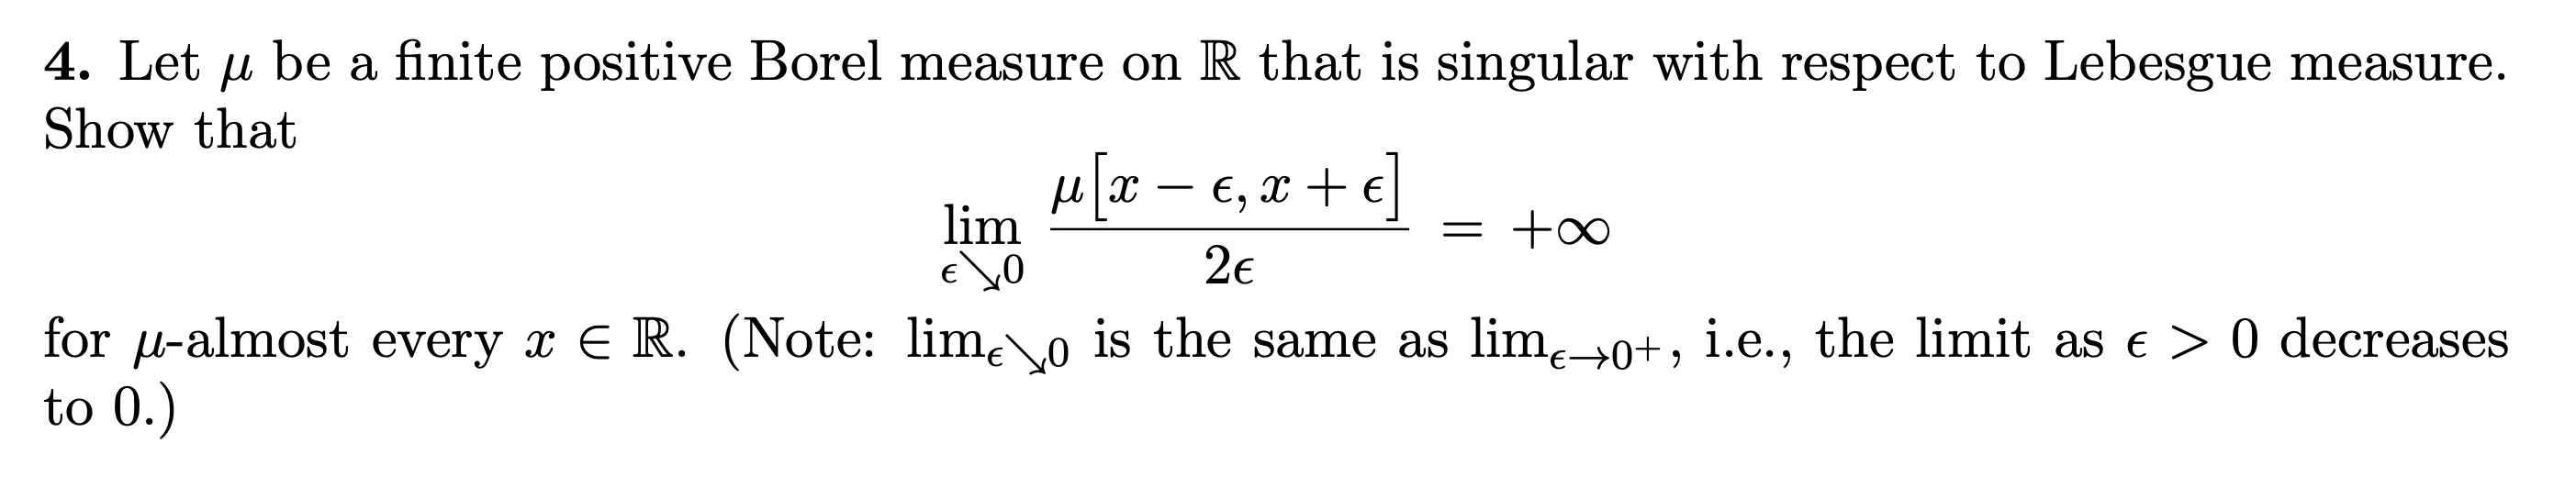
\includegraphics[width=400pt]{img/analysis--berkeley-202a-final-21a6.png}
\end{mdframed}

Let $m$ denote Lebesgue measure.

I am assuming that the question is saying that $\mu$ and $m$ are mutually singular with respect to the
Borel $\sigma$-algebra.

Intuition: in some sense this question is asking us to show that the Radon-Nikodym derivative does not exist,
because they are singular, which is sort of the opposite of absolutely continuous.

Intuition: $\mu$ assigns positive measure to a $m$-null set. Clearly we need to show that $\mu$ assigns greater
measure to certain intervals than $m$ does. Why is that true? Perhaps because the interval contains parts of
an $m$-null set.

In fact, $\mu$ only has positive measure on Lebesgue null sets. But $\mu$ does not assign positive measure to
every singleton, since $\mu$ is finite. If we could show that $\mu$-almost every $x$ is ``surrounded by an
arbitrarily small Lebesgue null set​'' that would do it. Perhaps the only way that makes sense is if
$\mu$-almost every $x$ is a singleton with positive measure under $\mu$. Can we show that?

$V$ contains no intervals, since it is Lebesgue-null. And $\mu(V) = L > 0$. This total measure $L$ is assigned
to Lebesgue-null sets in a countably additive manner.

\begin{mdframed}
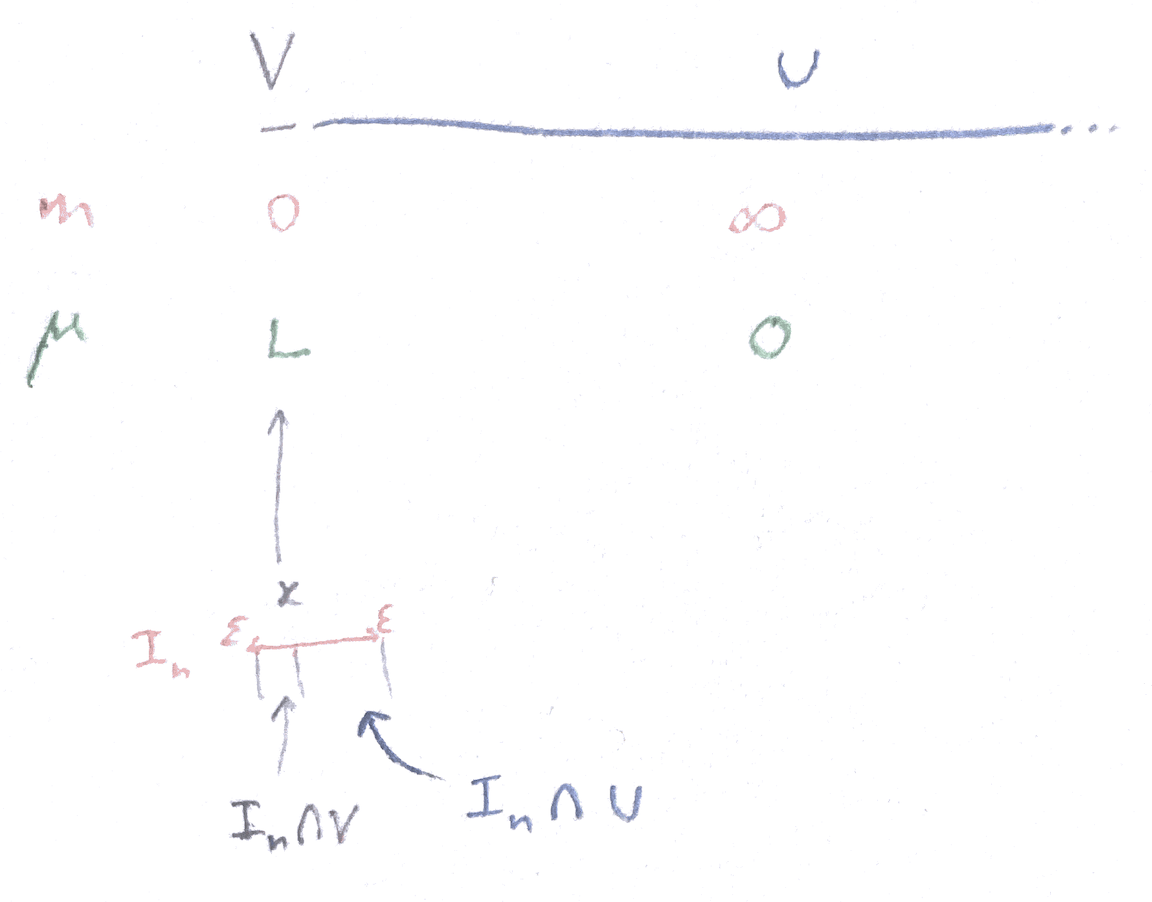
\includegraphics[width=400pt]{img/analysis--berkeley-202a-final-fe0f.png}
\end{mdframed}

\begin{proof}
  Since $\mu$ is singular with respect to Lebesgue measure, there exist disjoint Borel sets $U$ and $V$ such
  that $U$ is $\mu$-null and $V$ is $m$-null, and $\R = U \union V$.

  Let $0 < \mu(\R) = L < \infty$. We have
  \begin{align*}
    &\mu(U) = 0     & \mu(V) = L \\
    &m(U) = \infty & m(V) = 0,
  \end{align*}
  since by countable additivity $\infty = m(\R) = m(U) + m(V) = m(U)$,
  and $L = \mu(\R) = \mu(U) + \mu(V) = \mu(V)$.

  Note that any property that holds for all $x \in V$ holds $\mu$-almost everywhere. So let $x \in V$. We would
  like to show that
  \begin{align*}
    \lim_{\eps \searrow 0} \frac{\mu([x - \eps, x + \eps])}{2\eps} = +\infty.
  \end{align*}
  Let $\eps_n$ be a sequence converging to zero from above, let $I_n = [x - \eps_n, x + \eps_n]$, and
  let $B > 0$. We would like to show that there exists $N$ such that $\frac{\mu(I_n)}{2\eps_n} > B$ for
  all $n \geq N$.

  We have $\mu(I_n) = \mu(I_n \isect V) + \mu(I_n \isect U) = \mu(I_n \isect V)$, since $U$ is a null set
  under $\mu$. And since $x \in V$ we have $I_n \isect V \neq \emptyset$.

  My intuition is that as the interval $I_n$ gets smaller, it becomes enriched for points of $V$, which
  contribute positive measure to the numerator, and cause it to decrease more slowly than the denominator, in
  such a way that, for small enough $\eps$, the ratio exceeds any positive quantity $B$.

  If we could show that there exists $N$ and $l > 0$ such that $\mu(I_n) > l$ for all $n > N$ then we
  would be done, but that may not be true.

  I wonder whether we can discard a null set from $V$ so that our point $x$ is necessarily
\end{proof}


\newpage
\begin{mdframed}
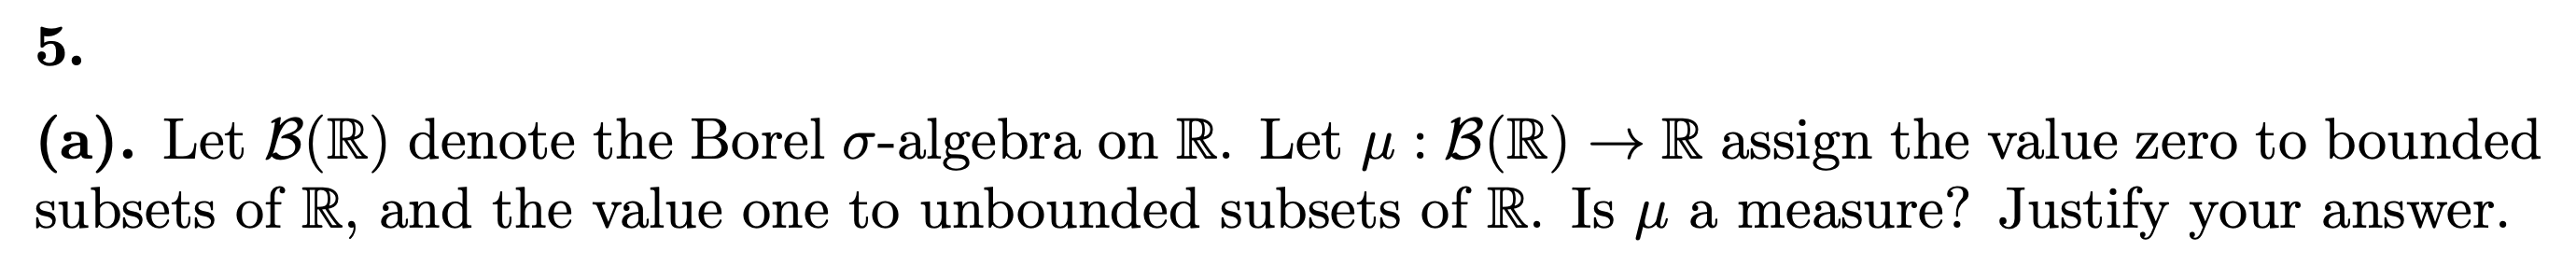
\includegraphics[width=400pt]{img/analysis--berkeley-202a-final-246a.png}
\end{mdframed}

\begin{proof}
  $\mu$ is not a measure because it is not countably additive.

  To see this, let $I_n = (-n, -(n - 1)] \union [n-1, n)$, and let $\mc I = \{I_n ~:~ n \in \N\}$. Then $\mc I$
  is a pairwise disjoint, countable collection of sets and $\bigcup_{n=1}^\infty \mc I = \R$,
  therefore $\mu\(\bigcup_{n=1}^\infty \mc I\) = 1$ since $\R$ is unbounded.

  However $I_n$ is bounded for all $n$ and
  so $\sum_{n=1}^\infty \mu(I_n) = \sum_{n=1}^\infty 0 = 0 \neq \mu\(\bigcup_{n=1}^\infty \mc I\)$.
\end{proof}


\begin{mdframed}
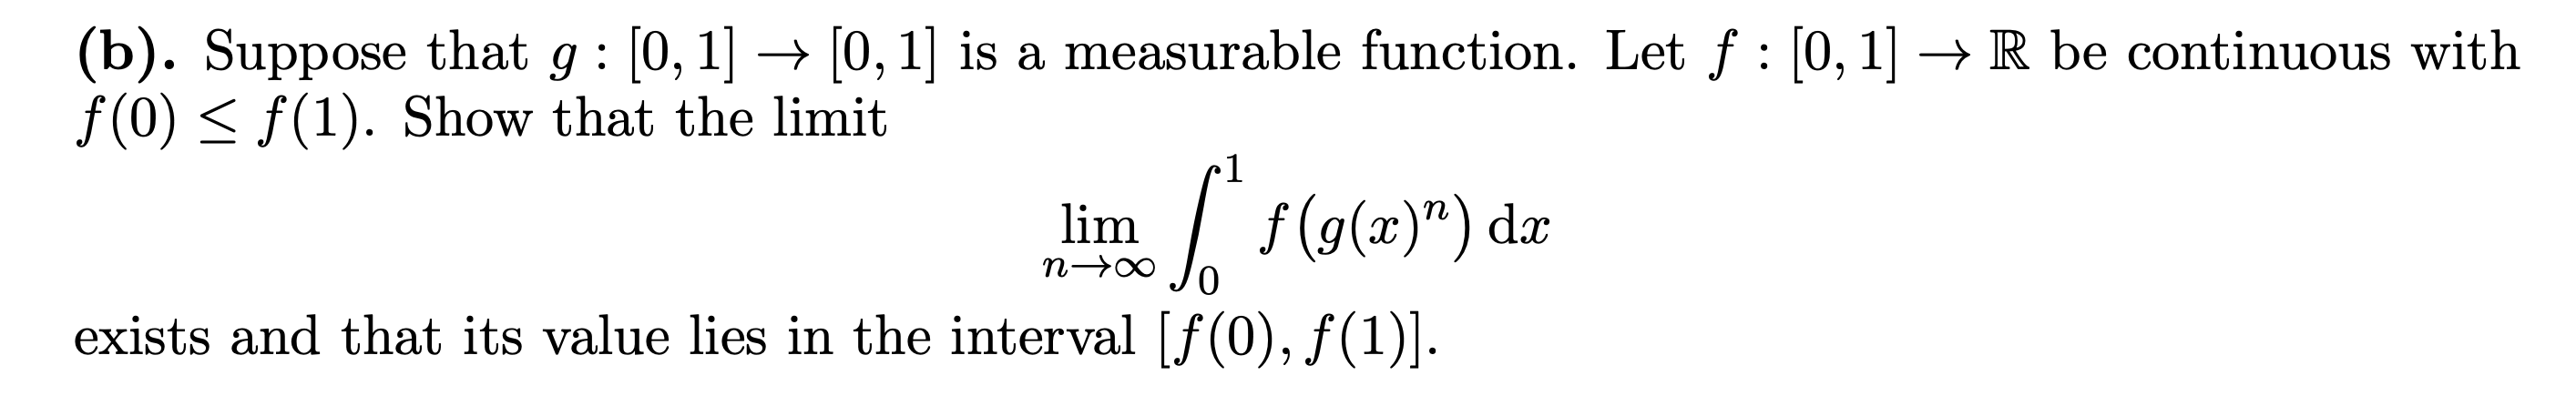
\includegraphics[width=400pt]{img/analysis--berkeley-202a-final-cd70.png}
\end{mdframed}

\begin{proof}
  Note that $f$ is continuous with compact support and so $f$ attains its bounds. Let $A = \inf f$
  and $B = \sup f$.

  Note that the integrand is bounded above by the constant integrable function $h(x) = B$ defined on $[0, 1]$.
  Therefore we may apply the dominated convergence theorem, yielding
  \begin{align*}
    \limninf \int_{[0, 1]} f(g(x)^n) \dx = \int_{[0, 1]} \limninf  f(g(x)^n) \dx.
  \end{align*}
  Let $U = g^{-1}(\{1\})$. We have $0 \leq g(x) \leq 1$ and therefore
  \begin{align*}
    \limninf g(x)^n =
    \begin{cases}
      1 & x \in U \\
      0 & \text{otherwise}.
    \end{cases}
  \end{align*}
  Since $g$ is measurable, $U$ is measurable, since it is a preimage of a measurable set. Let $\alpha = m(U)$.
  I believe that ``measurable​'' in the question refers to Lebesgue measure, so we have that $m([0, 1]) = 1$
  and $0 \leq \alpha \leq 1$. Therefore
  \begin{align*}
    \int_{[0, 1]} \limninf  f(g(x)^n) \dx
    &= \int_U \limninf  f(g(x)^n) \dx + \int_{[0, 1] \setminus U} \limninf  f(g(x)^n) \dx \\
    &= \int_U f(1) + \int_{[0, 1] \setminus U} f(0) \\
    &= \alpha f(1) + (1 - \alpha) f(0) \\
    &\in [f(0), f(1)].
  \end{align*}
\end{proof}


\newpage
\begin{mdframed}
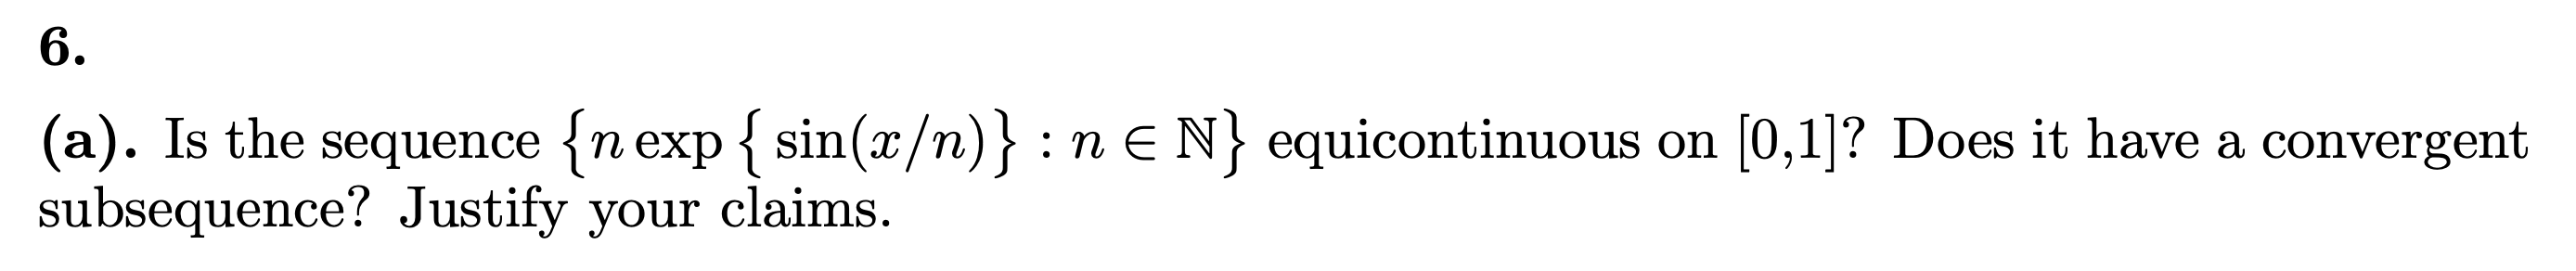
\includegraphics[width=400pt]{img/analysis--berkeley-202a-final-f5b6.png}
\end{mdframed}

\begin{mdframed}
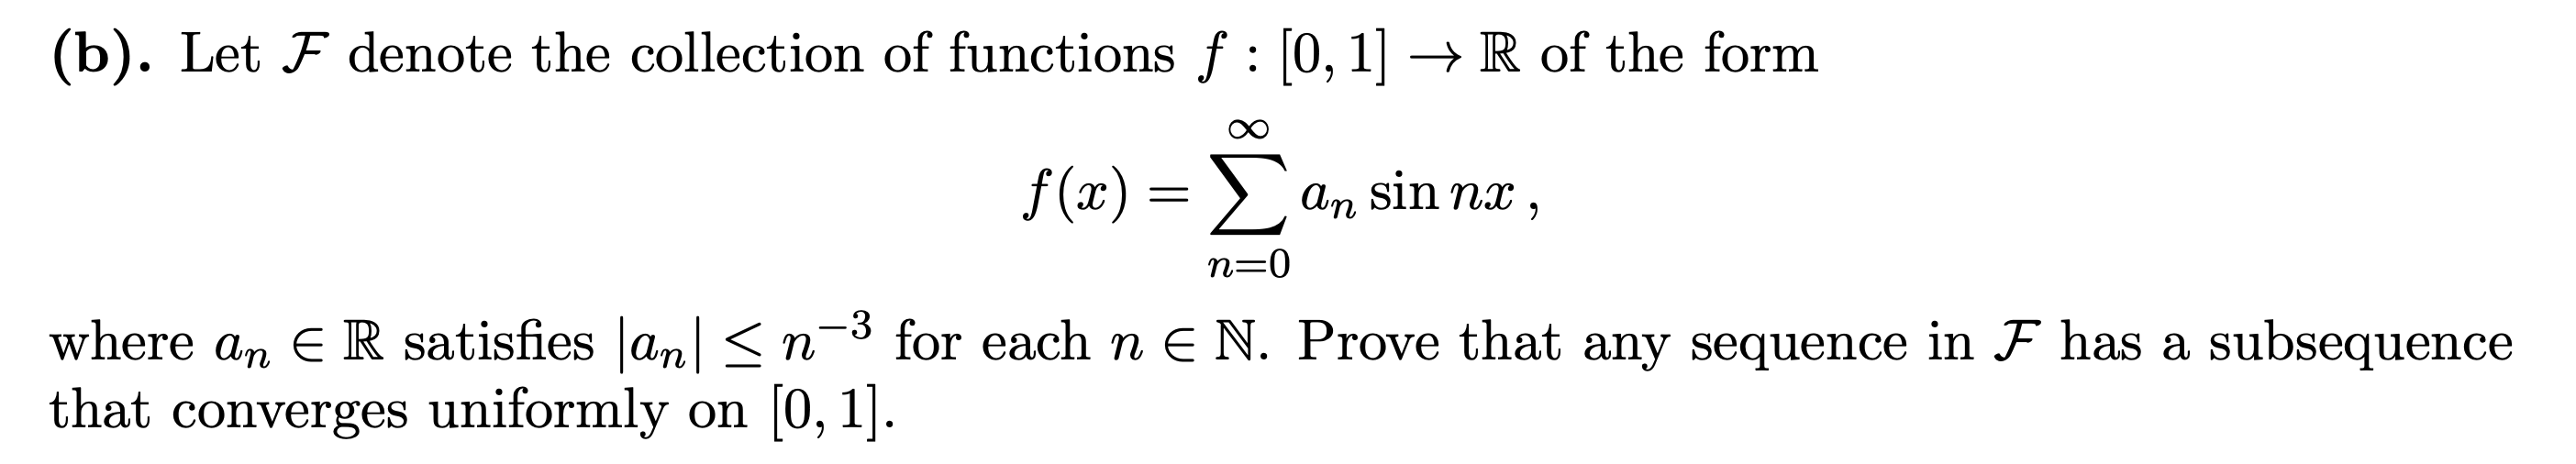
\includegraphics[width=400pt]{img/analysis--berkeley-202a-final-c7c7.png}
\end{mdframed}

\newpage
\begin{mdframed}
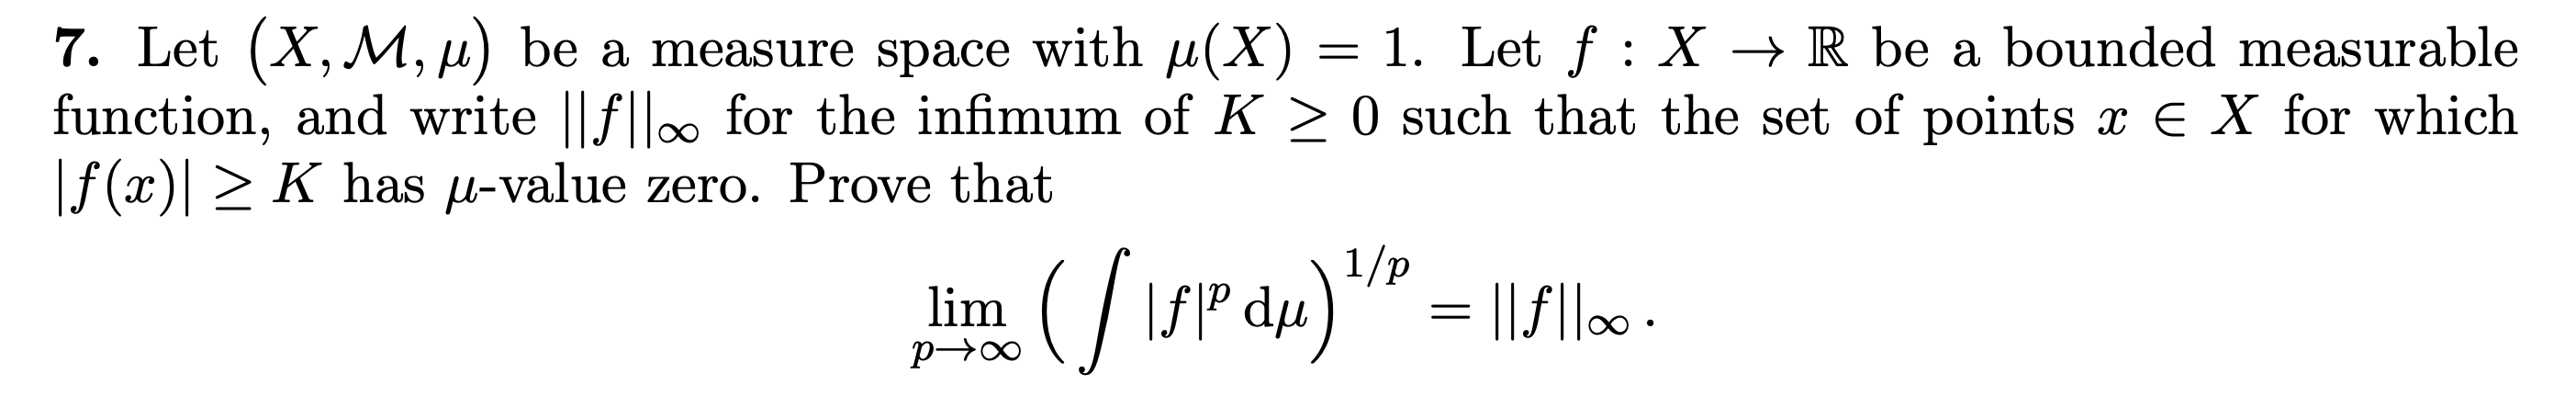
\includegraphics[width=400pt]{img/analysis--berkeley-202a-final-0000.png}
\end{mdframed}

\newpage
\begin{mdframed}
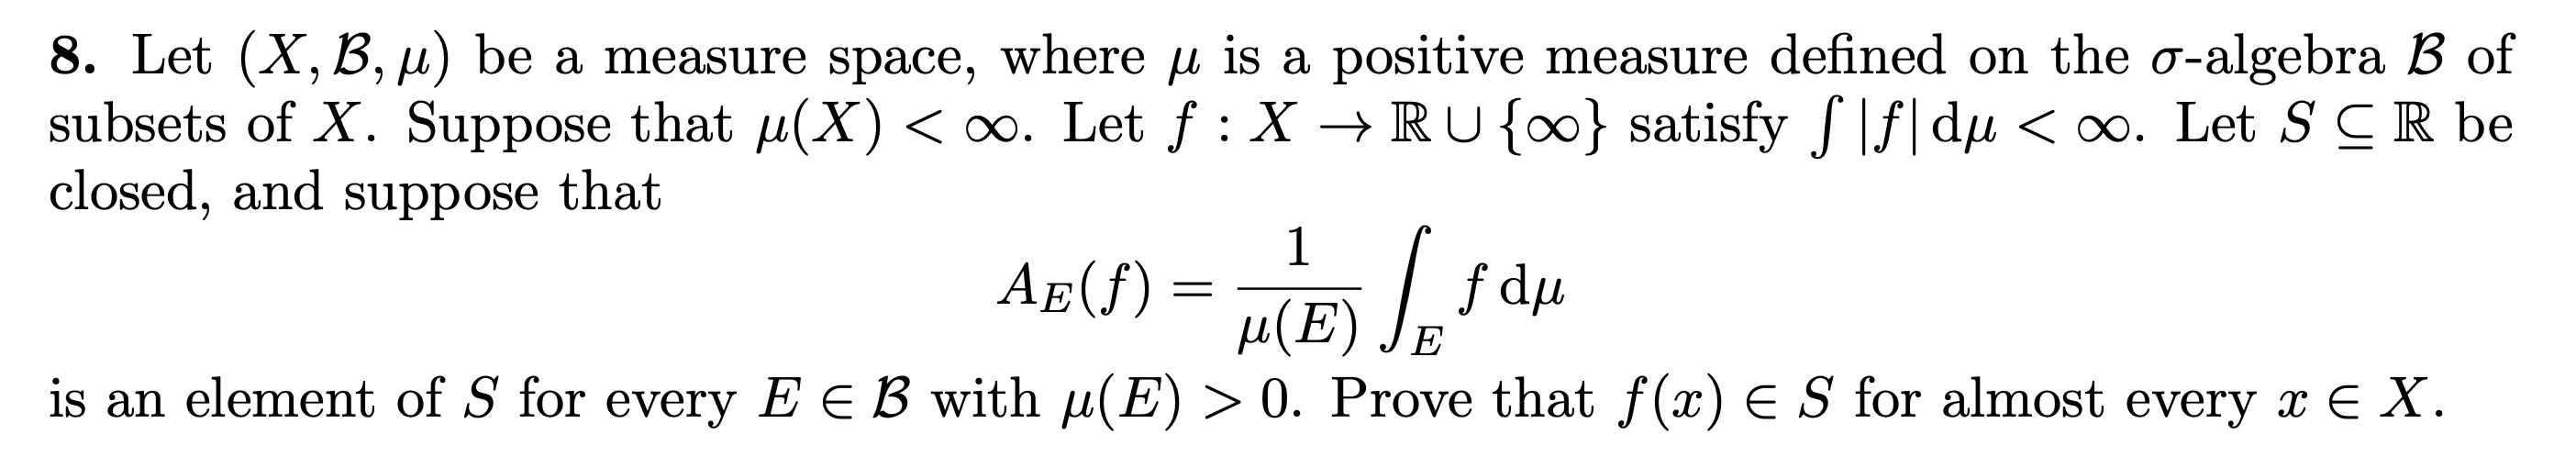
\includegraphics[width=400pt]{img/analysis--berkeley-202a-final-8aed.png}
\end{mdframed}
